\documentclass[a4paper]{article}
\usepackage[utf8]{inputenc}
\usepackage[spanish]{babel} 
\renewcommand{\spanishtablename}{Tabla} 
\spanishdecimal{.}
\usepackage{verbatim}
\usepackage{amssymb}
\usepackage{subcaption}
\usepackage{wrapfig}
\usepackage{graphicx}
\usepackage{hyperref}
\usepackage{mathtools}
\usepackage{float}
\usepackage{siunitx}
\renewcommand{\thefootnote}{\arabic{fotnote}}
\setlength{\parskip}{\baselineskip} 
\usepackage{pdfpages}

\begin{document}

\begin{titlepage}
\paragraph{}

\begin{center}
\vspace*{0.10in}
\begin{figure}
\raggedleft

\includegraphics[scale=0.12]{unam.png}
\hspace{7.2cm}
\raggedright

\includegraphics[scale=0.15]{fac.png}    
\end{figure}
\vspace*{0.5in}
UNIVERSIDAD NACIONAL AUTÓNOMA DE MÉXICO\\
\vspace*{0.2in}
FACULTAD DE CIENCIAS \\
\vspace*{0.5in}
\begin{large}
Laboratorio de Calor, Ondas y Fluidos\\
\end{large}
\vspace*{0.2in}
\begin{Large}
\textbf{Práctica 2} \\
\textbf{Ley de Enfriamiento} \\
\end{Large}
\vspace*{0.3in}
\vspace*{0.3in}
\rule{80mm}{0.1mm}\\
\vspace*{0.1in}
\begin{large}
Profesor:  Quintanar Robles, Luis  \\
Ayudante: Quintanar Cortés, Luis Enrique \\
Mesa 1\\
Fecha de la práctica: 27 de agosto de 2019.\\
Alumnos: León Arenal Sebastian.\\
Robledo Ibarra Emiliano. \\
Toledo Castañeda, Akim Tarik.\\

\end{large}
\end{center}
\end{titlepage}


\section{Resumen.}
Se buscó una relación entre el tiempo que tarda el agua en enfriarse y la masa del cuerpo de agua. Se calentaron diez masas distintas de agua a 50 grados Celsius y se monitoreó el tiempo de enfriamiento de cada una de ellas. En el experimento se encontró una relación directa: a mayor masa, más tiempo tarda en enfriarse (alcanzar equilibrio térmico con el ambiente); se encontró la constante que multiplica a la ecuación exponencial es cercana a la diferencia inicial de temperatura $(26.3\pm1.6)$ºC, la constante de linealización es el logaritmo natural de la diferencia $C = 3.30 \pm 0.04$ y la constante de proporcionalidad de la exponencial es dependiente de la masa que se está midiendo, a mayor masa menor es la constante y cercana a cero pero a menor masa más cercano es a uno.


%%%%%%%%%%%%%%%%%%%%%%%%%%%%%%%%%%%%%%%%%%%%%%%%%%%%%%%%%%%%%%%%%%%%%

\section{Introducción.}
El análisis térmico de un sistema es parte fundamental de sistemas dinámicos macroscópicos, un gran ejemplo de esta aplicación de modelaje es la meteorología: comúnmente se utiliza la ecuación de enfriamiento de Newton puesto que provee una aproximación bastante buena y sencilla al comportamiento de la temperie; conocer a qué temperatura ocurren los fenómenos termodinámicos es importante para su estudio por ejemplo: a qué temperatura hierve el agua, el punto de fusión de determinada sustancia pero qué ocurre si esta sustancia se calienta de más de lo necesario, ¿cuánto tiempo se tiene que esperar para que esta sustancia se encuentre a la temperatura deseada?, si se tiene una sustancia ¿se enfriará más rápido si es más masa o menos masa? Responder estas preguntas sería más fácil si se tuviera una relación entre la masa, el tiempo y la temperatura del cuerpo que se observa (llegar al equilibrio térmico con el ambiente). 

El objetivo de la práctica es confirmar experimentalmente que existe dicha relación entre la cantidad de sustancia que se tenga y el tiempo que esta se tarde en enfriar, en particular se utilizó el modelo simple de enfriamiento de sustancias relacionando tres variables: masa, temperatura y tiempo. La práctica consistió en calentar varias masas de agua a $50^{\circ}C$ y dejarlas enfriar a temperatura ambiente, anotando cuánto había decrecido la temperatura pasados 30$s$. Se formularon varias hipótesis con el fin de simplificar el experimento:
\begin{itemize}
    \item $1gr$ de agua $\equiv$ $1mL$ de agua. Esto es, su densidad es la ideal de 1$gr/cm^3$.
    \item La temperatura es homogénea en toda la masa de agua que se estudia.
\end{itemize}

Y las hipótesis que se aplicaron no sugieren una pérdida sustancial de rigor puesto que dichas aproximaciones son con frecuencia utilizadas, en cuanto a la densidad del agua, se ha medido que la variación es pequeña y no es significativa para temperaturas tan bajas como las que se usaron, para la segunda hipótesis se usó la ley cero de la termodinámica para un mismo sistema, que es sí mismo está a la misma temperatura. La primera hipótesis es valida para rangos de temperaturas bajos como los que se manejaron, sin embargo la segunda es válida para muchos sistemas.

%%%%%%%%%%%%%%%%%%%%%%%%%%%%%%%%%%%%%%%%%%%%%%%%%%%%%%%%%%%%%%%%%%%%%%

\section{Procedimiento.}

Con una probeta de 50mL se llenaron diez vasos de precipitados con agua. Se registraron volúmenes de $(200\pm 4)mL$, $(190\pm4)mL$, $(180\pm4)mL$, $(150\pm4)mL$, $(120\pm3)mL$, $(100\pm2)mL$, $(80\pm2)mL$, $(50\pm1)mL$, $(40\pm1)mL$ y $(20\pm1)mL$. Se corroboró con una balanza la masa de cada volumen para trabajar con los datos en gramos. Con una parrilla, se calentó cada masa a poco mas de $50^{\circ}C$. Una vez alcanzada esta temperatura, se retiró la masa de la fuente de calor y se agitó el vaso de precipitado para homogeneizar la temperatura del líquido. Con un termómetro bimetalico  se registraron las diferencias entre la temperatura ambiente y la temperatura del agua cada 30 segundos a partir de que el agua alcanzó los $(50.0\pm0.5)^{\circ}C$. Se dejó de registrar información cuando el agua alcanzó $(30.0\pm0.5)^{\circ}C$.

\begin{figure}[H]
    \centering
    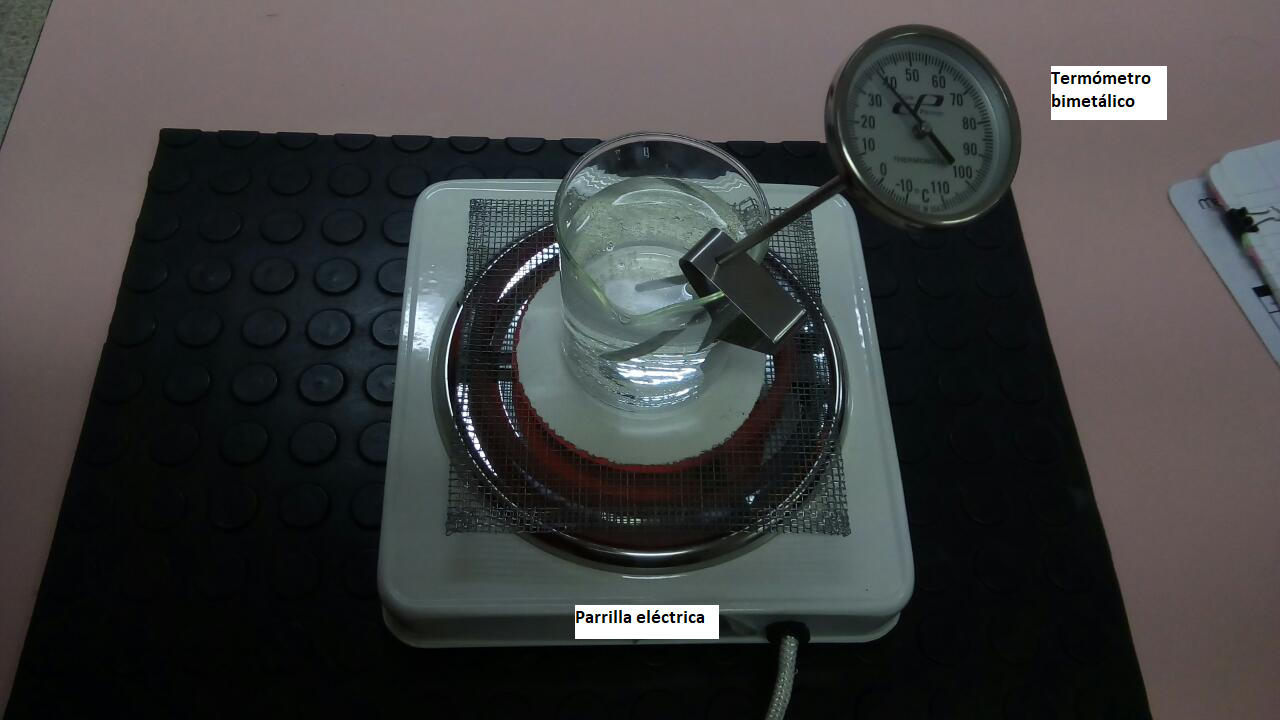
\includegraphics[width=11cm]{sist-2.png}% 
    \caption{Diagrama del sistema utilizado y sus elementos.}%
\end{figure}

En cuanto a la relación diferencia de temperatura contra tiempo se observó un comportamiento no lineal y los datos indican que decrece uniformemente pero conforme se acerca a la temperatura de estabilización el tiempo que toma al sistema es cada vez mayor, por ello a estos datos obtenidos a partir de la diferencia de temperaturas se les ajustó una función exponencial de la forma $f(x)=a*e^{-kx}$. Una vez ajustando los datos obtenidos, se buscó obtener el valor $k$ del ajuste y poder comprobar si la masa interviene; para darle linealidad a los datos, se aplicó logaritmo natural a la diferencia de temperaturas. Esta nueva relación ($Ln(\Delta T)$ contra $tiempo$) sí es de carácter lineal. Se observa que la "velocidad" del cambio de temperatura es proporcional a la diferencia entre la temperatura del sistema [$T_{s}$] y la temperatura ambiente [$T_{a}$]:

$$ \frac{\delta T}{\delta t} = -k(T_{s}-T_{a})$$

Donde k debe ser una constante positiva que dependa de la masa. El resultado debe ser negativo pues la temperatura está decreciendo en este experimento.
Manipulando esta expresión se puede llegar a:

$$\frac{\delta T}{T_{s}-T_{a}}= -k(\delta t)$$

E integrando ambos lados:

$$ Ln(T_{s}-T_{a})=-kt+C $$

Así pues, se llega a una ecuación lineal que relaciona la diferencia de temperaturas en el tiempo. Para el procesamiento de datos se utilizó GNUplot para aproximar valores a $k$ y $C$. 

Para tratar las incertidumbres en cada medición se consideraron los siguientes aspectos:
\begin{itemize}
    \item Los termómetros que se utilizaron para las medidas fueron bimetálicos lo cual arrojó una incertidumbre de 0.5ºC. Y para la diferencia de dos temperaturas se utilizó 1ºC ya que la temperatura ambiente se marcó en números enteros por la limitante del termómetro.
    \item Los volúmenes y masas se midieron con una probeta graduada que como resolución constaba de 2 mL, por ende su incertidumbre es de 1 mL. Y para mediciones más grandes se utilizó varias veces por lo cual dependiendo del volumen, se sumó tantas veces la incertidumbre como se usó.
    \item Para la linealización se aplicó la función logaritmo natural a las diferencias de temperaturas por lo que se utilizó la propagación de incertidumbres: $\left| \frac{1}{\Delta T} \right| (1)$. 
    \item En el caso de la incertidumbre del tiempo se consideró solamente un segundo que hizo el papel del retardo al cual se revisó el termómetro.
\end{itemize}

%%%%%%%%%%%%%%%%%%%%%%%%%%%%%%%%%%%%%%%%%%%%%%%%%%%%%%%%%%%%%%%%%
\section{Resultados.}
A continuación se colocan los datos obtenidos de las mediciones con una línea de tendencia, los datos se encuentran en el Apéndice:

\begin{figure}[H]
    \centering
    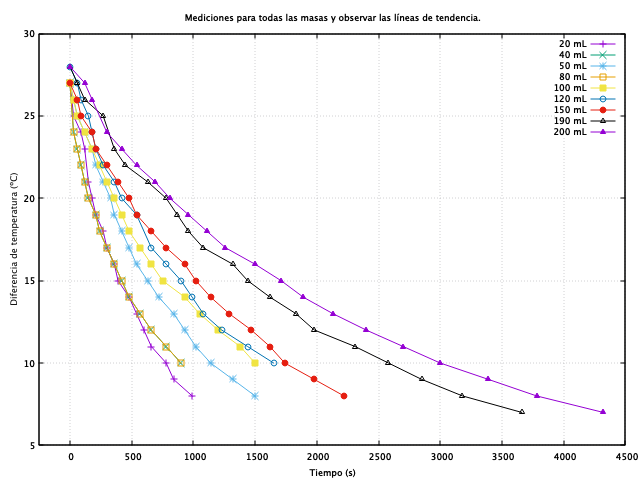
\includegraphics[width=11cm]{Todos.png}%
    \caption{Gráfica de todas las diferencias medidas unidas con su linea de tendencia.}%
\end{figure}

Una vez viendo la línea de tendencia se aplicó la función: $f(x) = a*e^{-x*b}$. Y los puntos resultan

\begin{figure}[H]
    \centering
    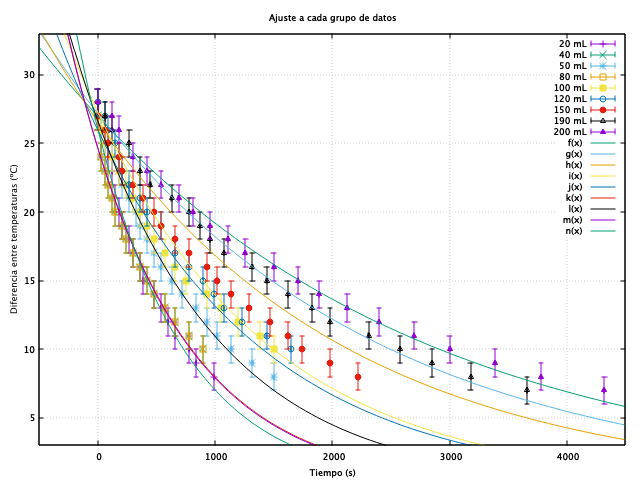
\includegraphics[width=11cm]{TODASALV.png}%
    \caption{Gráfica de todas las diferencias medidas unidas una función exponencial ajustada.}%
\end{figure}

\begin{itemize}
  \item Masa de $200 gr$: $a=(27.0\pm0.2)$; $b=(-341\times10^{-6} \pm 8\times 10^{-6})$.
  \item Masa de $190 gr$: $a=(27.2\pm0.2)$; $b=(-401\times10^{-6} \pm 7\times 10^{-6})$.
  \item Masa de $180 gr$: $a=(26.6\pm0.3)$; $b=(-45.7\times10^{-5} \pm 1.2\times 10^{-5})$.
  
  \item Masa de $150 gr$: $a=(26.33\pm0.14)$; $b=(-551\times10^{-6} \pm 8\times 10^{-6})$.
  \item Masa de $120 gr$: $a=(27.3\pm0.2)$; $b=(-67\times10^{-5} \pm 2\times 10^{-5})$.
  \item Masa de $100 gr$: $a=(26.0\pm0.2)$; $b=(-68\times10^{-5} \pm 2\times 10^{-5})$.
  \item Masa de $80 gr$: $a=(24.7\pm0.4)$; $b=(-113\times10^{-5} \pm 6\times 10^{-5})$.
  \item Masa de $50 gr$: $a=(26.67\pm0.14)$; $b=(-89.8\times10^{-5} \pm 1.5\times 10^{-5})$.
  \item Masa de $40 gr$: $a=(24.7\pm0.4)$; $b=(-114\times10^{-5} \pm 6\times 10^{-5})$.
  \item Masa de $20 gr$: $a=(26.1\pm0.3)$; $b=(-131\times10^{-5} \pm 4\times 10^{-5})$.
\end{itemize}

Una vez obtenida la tendencia exponencial se linealizaron los datos obtenidos aplicándoles el logaritmo natural de manera que los siguientes datos son en sí una recta: $m*x+b$.

\begin{figure}[H]
    \centering
    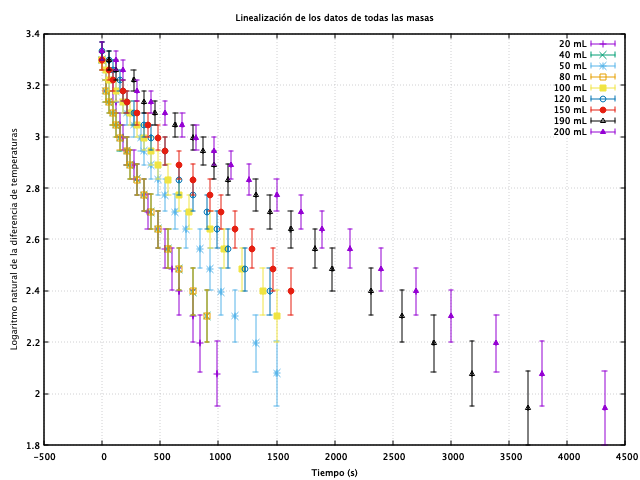
\includegraphics[width=11cm]{Lineali.png}%
    \caption{Linealización de la diferencia de temperaturas.}%
\end{figure}

\begin{itemize}
  \item Masa de $200 gr$: $m=(-340\times10^{-6}\pm8\times10^{-6})$; $b=(3.297\pm0.009)$.
  \item Masa de $190 gr$: $m=(-401\times10^{-6}\pm7\times10^{-6})$; $b=(3.304\pm0.008)$.
  \item Masa de $180 gr$: $m=(-48.0\times10^{-5}\pm1.4\times10^{-5})$;  $b=(3.292\pm0.009)$.
  \item Masa de $150 gr$: $m=(-55\times10^{-5}\pm1\times10^{-5})$;   $b=(3.272\pm0.006)$.
  \item Masa de $120 gr$: $m=(-68.4\times10^{-5}\pm1.6\times10^{-5})$; $b=(3.309\pm0.008)$.
  \item Masa de $100 gr$: $m=(-67.8\times10^{-5}\pm2\times10^{-5})$; $b=(3.258\pm0.009)$.
  \item Masa de $80 gr$:  $m=(-114\times10^{-5}\pm6\times10^{-5})$;   $b=(3.208\pm0.016)$.
  \item Masa de $50 gr$:  $m=(-86.1\times10^{-5}\pm1.4\times10^{-5})$; $b=(3.276\pm0.006)$.
  \item Masa de $40 gr$:  $m=(-113\times10^{-5}\pm6\times10^{-5})$;   $b=(3.208\pm0.016)$.
  \item Masa de $20 gr$:  $m=(-131\times10^{-5}\pm4\times10^{-5})$;   $b=(3.263\pm0.011)$.
\end{itemize}

\begin{figure}[H]
    \centering
    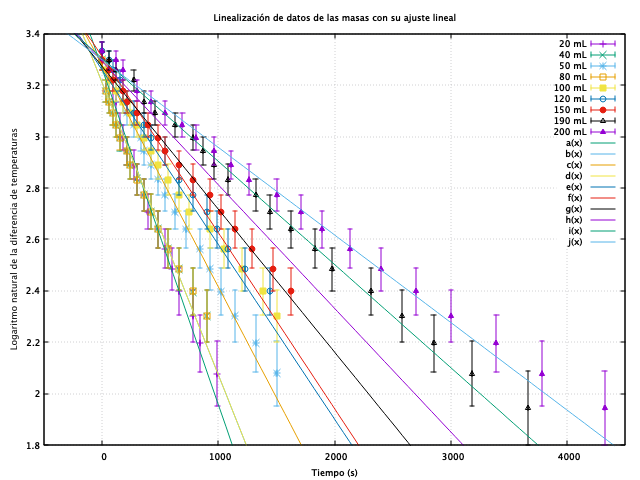
\includegraphics[width=11cm]{LINEASALV.png}%
    \caption{Lineas ajustadas a los datos que se les aplicó logaritmo natural.}%
\end{figure}






%%%%%%%%%%%%%%%%%%%%%%%%%%%%%%%%%%%%%%%%%%%%%%%%%%%%%%%%%%%%%%%%%

\section{Conclusiones.}

Las ecuaciones de función ajustada en "Figura 2'' es precisamente la función inversa a la ecuación lineal que involucra el logaritmo natural. Ciertamente, a mayor masa en el cuerpo de agua, mayor es el tiempo de enfriamiento de este. La constante supuesta $k$ se supuso en función de la masa; sin embargo, no es posible determinar sólo con este experimento si en realidad depende de la masa o de la masa y la sustancia seleccionada. Se requiere hacer el mismo procedimiento con distinta sustancias y comparar sus $k$.Para las masas pequeñas de agua se utilizaron vasos mas pequeños para contenerla y poder monitores su temperatura. Idealmente, todos las masas deberían estar sujetas a las mismas condiciones. Se desconoce el impacto que esto pueda tener en los resultados.

Se observó que en el primer ajuste el valor promedio del coeficiente que multiplica a la exponencial es cercano a la diferencia de temperaturas inicial $T_x - T_a = (50.0\pm0.5) - (23\pm0.5) C = (27\pm1)C$ y $\bar{a} = 26.26$, por lo cual se puede observar que hay cierta relación entre estas dos cantidades; al haber linealizado la función la ordenada al origen aparece como un nuevo número y de manera similar al caso anterior que todas sean semejantes y cercanas nos habla de una variable que se repitió en el experimento y la única que se intentó controlar fue la temperatura inicial y la ambiental con su diferencia, y este término, a saber $b$ (del ajuste lineal) es cercano a $ln(50-23) = (3.30\pm0.04)$ donde $\bar{b} = 3.26$. De forma análoga a las anteriores la pendiente que obtenemos de los ajustes lineales muestran una tendencia a uno conforme la masa se va reduciendo y esto es un resultado directo de los datos debido a que conforme las masas eran menores, más rápido fue su enfriamiento.

Un aspecto que resaltó fue que al linealizar los valores las incertidumbres más cercanos al cero, es decir mientras la diferencia se acercaba a cero, las incertidumbres dadas por la ecuación: $\left|\frac{1}{T_x - T_a} \right|$ se volvieron particularmente grandes; lo cual se explica con que la incertidumbre de la diferencia se vuelve relativamente mayor para estos valores, es por ello que en comparativa, los primeros datos para la linealización cuentan con una importancia mayor para mostrar tendencias y podrían descartarse algunos datos finales, sin embargo en el ajuste no afectaron lo suficiente puesto que GNUplot toma esto en cuenta y los errores no sobrepasaron el 5\%.

Por último, una limitante en las observaciones fue establecer un lapso para cada medición, es decir, si se busca un mejor modelo en cuanto a precisión  se debió tomar registro continuamente para una obtención de datos más sensibles y de comportamiento natural ya que al medir intervalos se sesga la información, sin embargo esta pérdida no fue significativa y no marcó un error en las mediciones en general.


\section{Apéndice.}
Aquí se colocan las tablas de las mediciones de la diferencia de temperaturas $T_x - T_a$:
% Table generated by Excel2LaTeX from sheet 'Sheet1'
\begin{table}[H]
  \centering
    \begin{tabular}{|c|c|c|c|} \hline
    Tiempo (s) & $T_x - T_a$ (ºC) & $s_{tiempo }$ & $s_{ \Delta T} $\\ \hline
    0     & 28    & 1     & 1 \\ \hline
    120   & 27    & 1     & 1 \\ \hline
    180   & 26    & 1     & 1 \\ \hline
    300   & 24    & 1     & 1 \\ \hline
    420   & 23    & 1     & 1 \\ \hline
    540   & 22    & 1     & 1 \\ \hline
    690   & 21    & 1     & 1 \\ \hline
    810   & 20    & 1     & 1 \\ \hline
    960   & 19    & 1     & 1 \\ \hline
    1110  & 18    & 1     & 1 \\ \hline
    1260  & 17    & 1     & 1 \\ \hline
    1500  & 16    & 1     & 1 \\ \hline
    1710  & 15    & 1     & 1 \\ \hline
    1890  & 14    & 1     & 1 \\ \hline
    2130  & 13    & 1     & 1 \\ \hline
    2400  & 12    & 1     & 1 \\ \hline
    2700  & 11    & 1     & 1 \\ \hline
    3000  & 10    & 1     & 1 \\ \hline
    3390  & 9     & 1     & 1 \\ \hline
    3780  & 8     & 1     & 1 \\ \hline
    4320  & 7     & 1     & 1 \\ \hline
    \end{tabular}%
  \caption{Tabla de la diferencias de temperaturas para la masa de $(200\pm 4)g$.}
\end{table}%

% Table generated by Excel2LaTeX from sheet 'Sheet1'
\begin{table}[H]
  \centering
    \begin{tabular}{|c|c|c|c|} \hline
    Tiempo (s) & $T_x - T_a$ (ºC) & $s_{tiempo }$ (s) &  $s_{ \Delta T} $(ºC) \\ \hline
    0     & 28    & 1     & 1 \\ \hline
    60    & 27    & 1     & 1 \\ \hline
    120   & 26    & 1     & 1 \\ \hline
    270   & 25    & 1     & 1 \\ \hline
    360   & 23    & 1     & 1 \\ \hline
    450   & 22    & 1     & 1 \\ \hline
    630   & 21    & 1     & 1 \\ \hline
    780   & 20    & 1     & 1 \\ \hline
    870   & 19    & 1     & 1 \\ \hline
    960   & 18    & 1     & 1 \\ \hline
    1080  & 17    & 1     & 1 \\ \hline
    1320  & 16    & 1     & 1 \\ \hline
    1440  & 15    & 1     & 1 \\ \hline
    1620  & 14    & 1     & 1 \\ \hline
    1830  & 13    & 1     & 1 \\ \hline
    1980  & 12    & 1     & 1 \\ \hline
    2310  & 11    & 1     & 1 \\ \hline
    2580  & 10    & 1     & 1 \\ \hline
    2850  & 9     & 1     & 1 \\ \hline
    3180  & 8     & 1     & 1 \\ \hline
    3660  & 7     & 1     & 1 \\ \hline
    \end{tabular}%
     \caption{Tabla de la diferencias de temperaturas para la masa de $(190\pm 4)g$.}
\end{table}%

% Table generated by Excel2LaTeX from sheet 'Sheet1'
\begin{table}[H]
  \centering
    \begin{tabular}{|c|c|c|c|} \hline
    Tiempo (s) & $T_x - T_a$ (ºC) & $s_{tiempo }$ (s) &  $s_{ \Delta T} $(ºC) \\ \hline
    0     & 28    & 1     & 1 \\ \hline
    30    & 27    & 1     & 1 \\ \hline
    90    & 26    & 1     & 1 \\ \hline
    180   & 25    & 1     & 1 \\ \hline
    270   & 23    & 1     & 1 \\ \hline
    360   & 22    & 1     & 1 \\ \hline
    450   & 21    & 1     & 1 \\ \hline
    540   & 20    & 1     & 1 \\ \hline
    660   & 19    & 1     & 1 \\ \hline
    780   & 18    & 1     & 1 \\ \hline
    930   & 17    & 1     & 1 \\ \hline
    1080  & 16    & 1     & 1 \\ \hline
    1230  & 15    & 1     & 1 \\ \hline
    1410  & 14    & 1     & 1 \\ \hline
    1560  & 13    & 1     & 1 \\ \hline
    1740  & 12    & 1     & 1 \\ \hline
    2010  & 11    & 1     & 1 \\ \hline
    2250  & 10    & 1     & 1 \\ \hline
    2490  & 9     & 1     & 1 \\ \hline
    2790  & 8     & 1     & 1 \\ \hline
    3210  & 7     & 1     & 1 \\ \hline
    \end{tabular}%
  \caption{Tabla de la diferencias de temperaturas para la masa de $(180\pm 4)g$.}
\end{table}%

% Table generated by Excel2LaTeX from sheet 'Sheet1'
\begin{table}[H]
  \centering
    \begin{tabular}{|c|c|c|c|} \hline
    Tiempo (s) & $T_x - T_a$ (ºC) & $s_{tiempo }$ (s) &  $s_{ \Delta T} $(ºC) \\ \hline
    0     & 27    & 1     & 1 \\ \hline
    60    & 26    & 1     & 1 \\ \hline
    90    & 25    & 1     & 1 \\ \hline
    180   & 24    & 1     & 1 \\ \hline
    210   & 23    & 1     & 1 \\ \hline
    300   & 22    & 1     & 1 \\ \hline
    390   & 21    & 1     & 1 \\ \hline
    480   & 20    & 1     & 1 \\ \hline
    540   & 19    & 1     & 1 \\ \hline
    660   & 18    & 1     & 1 \\ \hline
    780   & 17    & 1     & 1 \\ \hline
    930   & 16    & 1     & 1 \\ \hline
    1020  & 15    & 1     & 1 \\ \hline
    1140  & 14    & 1     & 1 \\ \hline
    1290  & 13    & 1     & 1 \\ \hline
    1470  & 12    & 1     & 1 \\ \hline
    1620  & 11    & 1     & 1 \\ \hline
    1740  & 10    & 1     & 1 \\ \hline
    1980  & 9     & 1     & 1 \\ \hline
    2220  & 8     & 1     & 1 \\ \hline
    \end{tabular}%
  \caption{Tabla de la diferencias de temperaturas para la masa de $(150\pm 3)g$.}
\end{table}%

% Table generated by Excel2LaTeX from sheet 'Sheet1'
\begin{table}[H]
  \centering
    \begin{tabular}{|c|c|c|c|} \hline
    Tiempo (s) & $T_x - T_a$ (ºC) & $s_{tiempo }$ (s) &  $s_{ \Delta T} $(ºC) \\ \hline
    0     & 28    & 1     & 1 \\ \hline
    60    & 27    & 1     & 1 \\ \hline
    90    & 26    & 1     & 1 \\ \hline
    150   & 25    & 1     & 1 \\ \hline
    180   & 24    & 1     & 1 \\ \hline
    210   & 23    & 1     & 1 \\ \hline
    270   & 22    & 1     & 1 \\ \hline
    360   & 21    & 1     & 1 \\ \hline
    420   & 20    & 1     & 1 \\ \hline
    540   & 19    & 1     & 1 \\ \hline
    660   & 17    & 1     & 1 \\ \hline
    780   & 16    & 1     & 1 \\ \hline
    900   & 15    & 1     & 1 \\ \hline
    990   & 14    & 1     & 1 \\ \hline
    1080  & 13    & 1     & 1 \\ \hline
    1230  & 12    & 1     & 1 \\ \hline
    1440  & 11    & 1     & 1 \\ \hline
    1650  & 10    & 1     & 1 \\ \hline
    \end{tabular}%
  \caption{Tabla de la diferencias de temperaturas para la masa de $(120\pm 3)g$.}
\end{table}%


% Table generated by Excel2LaTeX from sheet 'Sheet1'
\begin{table}[H]
  \centering
    \begin{tabular}{|c|c|c|c|} \hline
    Tiempo (s) & $T_x - T_a$ (ºC) & $s_{tiempo }$ (s) &  $s_{ \Delta T} $(ºC) \\ \hline
    0     & 27    & 1     & 1 \\ \hline
    30    & 26    & 1     & 1 \\ \hline
    60    & 25    & 1     & 1 \\ \hline
    120   & 24    & 1     & 1 \\ \hline
    180   & 23    & 1     & 1 \\ \hline
    240   & 22    & 1     & 1 \\ \hline
    300   & 21    & 1     & 1 \\ \hline
    360   & 20    & 1     & 1 \\ \hline
    420   & 19    & 1     & 1 \\ \hline
    480   & 18    & 1     & 1 \\ \hline
    570   & 17    & 1     & 1 \\ \hline
    660   & 16    & 1     & 1 \\ \hline
    750   & 15    & 1     & 1 \\ \hline
    930   & 14    & 1     & 1 \\ \hline
    1050  & 13    & 1     & 1 \\ \hline
    1200  & 12    & 1     & 1 \\ \hline
    1380  & 11    & 1     & 1 \\ \hline
    1500  & 10    & 1     & 1 \\ \hline
    \end{tabular}%
  \caption{Tabla de la diferencias de temperaturas para la masa de $(100\pm 2)g$.}
\end{table}%

% Table generated by Excel2LaTeX from sheet 'Sheet1'
\begin{table}[H]
  \centering
    \begin{tabular}{|c|c|c|c|} \hline
    Tiempo (s) & $T_x - T_a$ (ºC) & $s_{tiempo }$ (s) &  $s_{ \Delta T} $(ºC) \\ \hline
    0     & 27    & 1     & 1 \\ \hline
    30    & 24    & 1     & 1 \\ \hline
    60    & 23    & 1     & 1 \\ \hline
    90    & 22    & 1     & 1 \\ \hline
    120   & 21    & 1     & 1 \\ \hline
    150   & 20    & 1     & 1 \\ \hline
    210   & 19    & 1     & 1 \\ \hline
    240   & 18    & 1     & 1 \\ \hline
    300   & 17    & 1     & 1 \\ \hline
    360   & 16    & 1     & 1 \\ \hline
    420   & 15    & 1     & 1 \\ \hline
    480   & 14    & 1     & 1 \\ \hline
    570   & 13    & 1     & 1 \\ \hline
    660   & 12    & 1     & 1 \\ \hline
    780   & 11    & 1     & 1 \\ \hline
    900   & 10    & 1     & 1 \\ \hline
    \end{tabular}%
  \caption{Tabla de la diferencias de temperaturas para la masa de $(80\pm 2)g$.}
\end{table}%

% Table generated by Excel2LaTeX from sheet 'Sheet1'
\begin{table}[H]
  \centering
    \begin{tabular}{|c|c|c|c|} \hline
    Tiempo (s) & $T_x - T_a$ (ºC) & $s_{tiempo }$ (s) &  $s_{ \Delta T} $(ºC) \\ \hline
    0     & 27    & 1     & 1 \\ \hline
    30    & 26    & 1     & 1 \\ \hline
    60    & 25    & 1     & 1 \\ \hline
    120   & 24    & 1     & 1 \\ \hline
    180   & 23    & 1     & 1 \\ \hline
    210   & 22    & 1     & 1 \\ \hline
    270   & 21    & 1     & 1 \\ \hline
    330   & 20    & 1     & 1 \\ \hline
    360   & 19    & 1     & 1 \\ \hline
    420   & 18    & 1     & 1 \\ \hline
    480   & 17    & 1     & 1 \\ \hline
    540   & 16    & 1     & 1 \\ \hline
    630   & 15    & 1     & 1 \\ \hline
    720   & 14    & 1     & 1 \\ \hline
    840   & 13    & 1     & 1 \\ \hline
    930   & 12    & 1     & 1 \\ \hline
    1020  & 11    & 1     & 1 \\ \hline
    1140  & 10    & 1     & 1 \\ \hline
    1320  & 9     & 1     & 1 \\ \hline
    1500  & 8     & 1     & 1 \\ \hline
    \end{tabular}%
  \caption{Tabla de la diferencias de temperaturas para la masa de $(50\pm 1)g$.}
\end{table}%

% Table generated by Excel2LaTeX from sheet 'Sheet1'
\begin{table}[H]
  \centering
    \begin{tabular}{|c|c|c|c|} \hline
    Tiempo (s) & $T_x - T_a$ (ºC) & $s_{tiempo }$ (s) &  $s_{ \Delta T} $(ºC) \\ \hline
    0     & 27    & 1     & 1 \\ \hline
    30    & 24    & 1     & 1 \\ \hline
    60    & 23    & 1     & 1 \\ \hline
    90    & 22    & 1     & 1 \\ \hline
    120   & 21    & 1     & 1 \\ \hline
    150   & 20    & 1     & 1 \\ \hline
    210   & 19    & 1     & 1 \\ \hline
    240   & 18    & 1     & 1 \\ \hline
    300   & 17    & 1     & 1 \\ \hline
    360   & 16    & 1     & 1 \\ \hline
    420   & 15    & 1     & 1 \\ \hline
    480   & 14    & 1     & 1 \\ \hline
    570   & 13    & 1     & 1 \\ \hline
    660   & 12    & 1     & 1 \\ \hline
    780   & 11    & 1     & 1 \\ \hline
    900   & 10    & 1     & 1 \\ \hline
    \end{tabular}%
  \caption{Tabla de la diferencias de temperaturas para la masa de $(40\pm 1)g$.}
\end{table}%

% Table generated by Excel2LaTeX from sheet 'Sheet1'
\begin{table}[H]
  \centering
    \begin{tabular}{|c|c|c|c|} \hline
    Tiempo (s) & $T_x - T_a$ (ºC) & $s_{tiempo }$ (s) &  $s_{ \Delta T} $(ºC) \\ \hline
    0     & 27    & 1     & 1 \\ \hline
    30    & 25    & 1     & 1 \\ \hline
    90    & 24    & 1     & 1 \\ \hline
    120   & 23    & 1     & 1 \\ \hline
    150   & 21    & 1     & 1 \\ \hline
    180   & 20    & 1     & 1 \\ \hline
    210   & 19    & 1     & 1 \\ \hline
    270   & 18    & 1     & 1 \\ \hline
    300   & 17    & 1     & 1 \\ \hline
    360   & 16    & 1     & 1 \\ \hline
    390   & 15    & 1     & 1 \\ \hline
    480   & 14    & 1     & 1 \\ \hline
    540   & 13    & 1     & 1 \\ \hline
    600   & 12    & 1     & 1 \\ \hline
    660   & 11    & 1     & 1 \\ \hline
    780   & 10    & 1     & 1 \\ \hline
    840   & 9     & 1     & 1 \\ \hline
    990   & 8     & 1     & 1 \\ \hline
    \end{tabular}%
  \caption{Tabla de la diferencias de temperaturas para la masa de $(20\pm 1)g$.}
\end{table}%








\end{document}
